\documentclass[parskip=full]{scrartcl}
\usepackage{ucs}
\usepackage[german]{babel}  % german hyphenation, quotes, etc
\usepackage[utf8]{inputenc} % use utf8 file encoding for TeX sources
\usepackage[T1]{fontenc}    % avoid garbled Unicode text in pdf
\usepackage{hyperref}       % detailed hyperlink/pdf configuration
\hypersetup{                % ‘texdoc hyperref‘ for options
pdftitle={SWT1: Lastenheft},%
bookmarks=true,%
}
\usepackage{graphicx}       % provides commands for including figures
\usepackage{csquotes}       % provides \enquote{} macro for "quotes"
\usepackage[nonumberlist]{glossaries}     % provides glossary commands
\usepackage{enumitem}

\makenoidxglossaries

\newglossaryentry{Smartphone}
{
	name=Smartphone,
	plural=Smartphone,
	description={Mobiltelefon, welches \"uber das Telefonieren hinaus weitere Funktionalit\"aten beinhaltet, wie beispielsweise Internetzugang, Kamera oder Foto- und Videoaufnahmen},
}

\newglossaryentry{App}
{
	name=App,
	plural=App,
	description={Kleine Anwendungen, welche auf ein Smartphone heruntergeladen werden k\"onnen, bzw. teils schon vorinstalliert sind},
}

\newglossaryentry{Filter}
{
	name=Filter,
	plural=Filter,
	description={Voreingestellte und festgelegte Werte oder Effekte, welche auf ein digitales Bild angewandt werden k\"onnen. Das Bild hat dann seinen Orginalzustand abgelegt und hat nun z.B. verst\"arkte Rot-T\"one oder verwaschene Konturen},
}

\newglossaryentry{Google PlayStore}
{
	name=Google PlayStore,
	plural=-,
	description={Online-Markt der Firma 'Google', auf welchem App's f\"ur Android-Ger\"ate erworben und heruntergeladen werden k\"onnen},
}

\newglossaryentry{iOS App Store}
{
	name=iOS App Store,
	plural=-,
	description={Online-Markt der Firma 'Apple', auf welchem App's f\"ur iOS-Ger\"ate erworben und heruntergeladen werden k\"onnen},
}

\newglossaryentry{In-App Kauf}
{
	name=In-App Kauf,
	plural=In-App K\"aufe,
	description={Funktion, neue bzw. weitere Inhalte einer App k\"auflich zu erwerben. Dies geschieht meist per Zugriff auf das jeweilige App-Store-Konto, welches meist mit einer Zahlungsmethode online verkn\"upft ist},
}

\newglossaryentry{Primitiv}
{
	name=Primitiv,
	plural=Primitive,
	description={Bezeichnet elementare ein-, zwei- oder dreidimensionale geometrische Formen. (In diesem Fall zweidimensional.)}
}

\newglossaryentry{Server}
{
	name=Server,
	plural=Server,
	description={Rechnerstruktur, welche als Datenknoten und -verwaltungspunkt agiert}
}
	

\title{Lastenheft iMage}
\subtitle{Kunstfilter Plug-In}
\author{Jakob Dr\"ager, 2069436}

\begin{document}
\maketitle

\section{Zielbestimmung}
Das Produkt, die Kunstfilter-\glspl{App} 'iMage' der Firma Pear Corp. soll \"uber die M\"oglichkeit verf\"ugen, einzelne \glspl{Filter} auf Bilder anzuwenden und zu verwalten. Die \glspl{App} soll in einer Basis-Variante ausgeliefert werden, welche den \glspl{Filter} 'Geometrify' enth\"alt.

\section{Produkteinsatz}
 Der Vertrieb der \glspl{Smartphone}-\glspl{App} soll also \"uber den '\glspl{Google PlayStore}' und den '\glspl{iOS App Store}' erfolgen. Hierbei soll die Funktion des '\glspl{In-App Kauf}s' in den jeweiligen M\"arkten dazu genutzt werden, weitere Filter den Nutzern gegen Aufpreis anzubieten.
 
Zielgruppe: Nutzer des \glspl{Smartphone}s als Kamera bzw. zur mobilen und schnellen Bildbearbeitung.

Plattform: \glspl{Smartphone}s mit dem Betriebsystem Android oder iOS.

\section{Funktionale Anforderungen}
\begin{itemize}[nosep]
\item[FA10] Der mitgelieferte \glspl{Filter} 'Geometrify' soll in der Lage sein, ein gegebenes Bild durch Hinzuf\"ugen vieler gleichartiger \glspl{Primitiv}e nachzubilden. Hierbei soll das verwendete \glspl{Primitiv} gew\"ahlt werden k\"onnen.
\item[FA20] Die Auswahl soll per Auswahlmen\"u in der graphischen Benutzeroberfl\"ache von iMage erm\"oglicht werden.
\item[FA30] Nach der Auswahl des \glspl{Primitiv}s soll eine Vorschau des \glspl{Filter}effektes f\"ur das aktuelle Bild angezeigt werden.
\item[FA40] Die Berechnung des Vorschaubilds soll in Echtzeit m\"oglich sein.
\item[FA50] Hierzu soll beim Laden des Bilds durch den Nutzer zus\"atzlich eine Variante mit niedriger Aufl\"osung abgespeichert werden.
\item[FA60] Nach der Beendigung der \glspl{App} sollen diese Bilder zur Verbesserung der \glspl{App} an die Pear-Corp.-Firmenzentrale \"ubermittelt werden.
\end{itemize}

\section{Produktdaten}
\begin{itemize}[nosep]
\item[PD10] Es soll eine Ansicht \"uber alle get\"atigten In-App K\"aufe geben.
\item[PD20] Es soll die M\"oglichkeit geben, alte K\"aufe auf neuen Ger\"aten wieder herzustellen.
\item[PD30] Es sollen relevante Zahlungsdaten der Nutzer auf dem Ger\"at gespeichert werden.
\end{itemize}

\section{Nichtfunktionale Anforderungen}
\begin{itemize}[nosep]
\item[NF10] Es sollen, pro Ver\"offentlichung von neuen \glspl{Filter}n, mindestens 2000 In-App-K\"aufe get\"atigt werden.
\item[NF20] Die App soll regelm\"assig den firmeneigenen \glspl{Server} nach neuen Angeboten abfragen.
\item[NF30] Zahlungsdaten der Nutzer m\"ussen verschl\"usselt gespeichert sein.
\item[NF40] Bei saisonalen Angeboten soll die Ersparnis gegen\"uber dem Einzelerwerb der Bestandteile anzeigt werden.
\end{itemize}

\newpage

\section{Systemmodelle}

\subsection{Anwendungsf\"alle}
'In-App-Kauf' - System
\begin{center}
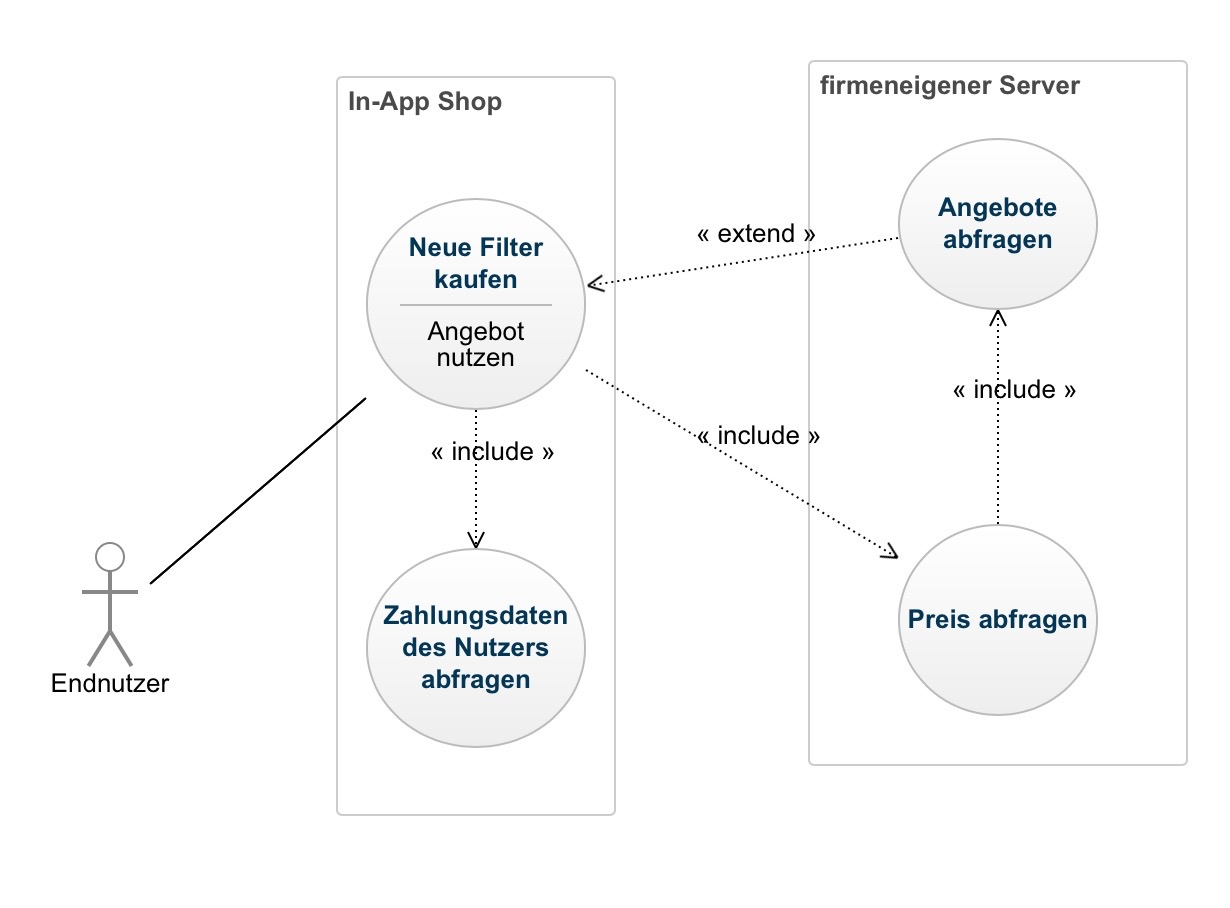
\includegraphics[width=1\textwidth]{In-App-Kauf-System.jpg}
\end{center}

\glsaddall
\printnoidxglossaries

\end{document}